\documentclass[border=4pt]{standalone}
\usepackage{fontspec}
\setmainfont{DMSans9pt}[Path=../../fonts/, Extension=.ttf, UprightFont=*-Regular, BoldFont=*-Bold, ItalicFont=*-Italic, BoldItalicFont=*-BoldItalic]
\setsansfont{DMSans9pt}[Path=../../fonts/, Extension=.ttf, UprightFont=*-Regular, BoldFont=*-Bold, ItalicFont=*-Italic, BoldItalicFont=*-BoldItalic]
\usepackage{amsmath,amssymb,xcolor,adjustbox,pifont}
\usepackage{tikz}
\usetikzlibrary{arrows.meta,positioning,shapes.geometric,shapes.misc,fit,backgrounds,calc,decorations.pathreplacing,shadows}
\usepackage[edges]{forest}
\usepackage{pgfplots}
\pgfplotsset{compat=1.18}

%% ---------- colours and macros used throughout
\definecolor{cTwo}{HTML}{4C72B0}   % two-stage
\definecolor{cOne}{HTML}{DD8452}   % one-stage / YOLO
\definecolor{cDetr}{HTML}{55A868}  % DETR
\definecolor{cOvd}{HTML}{8172B3}   % open-vocabulary
\definecolor{cAgent}{HTML}{C44E52} % agentic
\definecolor{cEdge}{HTML}{937860}  % edge
\definecolor{cApp}{HTML}{DA8BC3}   % applications
\definecolor{cData}{HTML}{4C9BB0}  % data / metrics
\newcommand{\tleaf}[1]{\parbox{8.3cm}{\raggedright #1}}
\newcommand{\tmid}[1]{\parbox{2.9cm}{\raggedright #1}}
\newcommand{\tone}[1]{\parbox{2.3cm}{\raggedright #1}}
\newcommand{\cmark}{\ding{51}}
\newcommand{\xmark}{\ding{55}}
\newcommand{\pmark}{$\circ$}


\renewcommand{\cite}[1]{}
\providecommand{\ref}[1]{}
\renewcommand{\ref}[1]{}
\newcommand{\tbd}[1]{#1}
\begin{document}
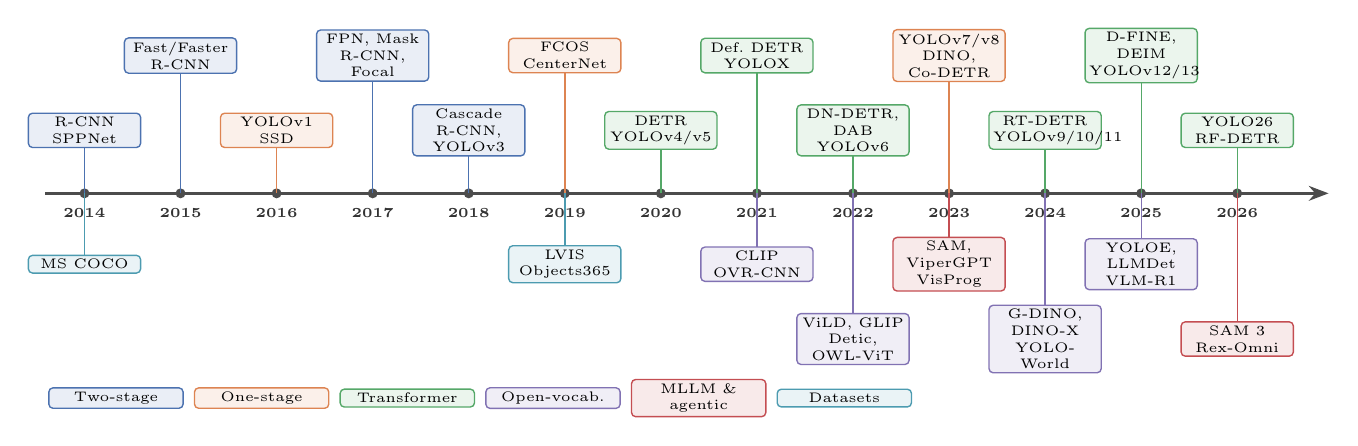
\begin{tikzpicture}[
  yr/.style={font=\bfseries\tiny, text=black!80},
  ev/.style={font=\tiny, align=center, rounded corners=1.5pt, inner sep=1.5pt, text width=1.32cm, draw=#1, fill=#1!12, line width=0.5pt},
  conn/.style={draw=#1, line width=0.5pt}
]
\def\dx{1.22}
\draw[-{Stealth[length=2.5mm]}, line width=1.2pt, black!70] (0,0) -- (16.3,0);
\foreach \y [count=\i from 0] in {2014,2015,2016,2017,2018,2019,2020,2021,2022,2023,2024,2025,2026}{
  \pgfmathsetmacro\x{0.5+\i*\dx}
  \fill[black!70] (\x,0) circle (1.8pt);
  \node[yr] at (\x,-0.25) {\y};
}
\newcommand{\evt}[4]{%
  \pgfmathsetmacro\xx{0.5+#1*\dx}
  \draw[conn=#3] (\xx,0) -- (\xx,#2);
  \node[ev=#3] at (\xx,#2) {#4};
}
\evt{0}{0.8}{cTwo}{R-CNN\\SPPNet}
\evt{1}{1.75}{cTwo}{Fast/Faster\\R-CNN}
\evt{2}{0.8}{cOne}{YOLOv1\\SSD}
\evt{3}{1.75}{cTwo}{FPN, Mask\\R-CNN, Focal}
\evt{4}{0.8}{cTwo}{Cascade\\R-CNN, YOLOv3}
\evt{5}{1.75}{cOne}{FCOS\\CenterNet}
\evt{6}{0.8}{cDetr}{DETR\\YOLOv4/v5}
\evt{7}{1.75}{cDetr}{Def.\ DETR\\YOLOX}
\evt{8}{0.8}{cDetr}{DN-DETR, DAB\\YOLOv6}
\evt{9}{1.75}{cOne}{YOLOv7/v8\\DINO, Co-DETR}
\evt{10}{0.8}{cDetr}{RT-DETR\\YOLOv9/10/11}
\evt{11}{1.75}{cDetr}{D-FINE, DEIM\\YOLOv12/13}
\evt{12}{0.8}{cDetr}{YOLO26\\RF-DETR}
\evt{0}{-0.9}{cData}{MS COCO}
\evt{5}{-0.9}{cData}{LVIS\\Objects365}
\evt{7}{-0.9}{cOvd}{CLIP\\OVR-CNN}
\evt{8}{-1.85}{cOvd}{ViLD, GLIP\\Detic, OWL-ViT}
\evt{9}{-0.9}{cAgent}{SAM, ViperGPT\\VisProg}
\evt{10}{-1.85}{cOvd}{G-DINO, DINO-X\\YOLO-World}
\evt{11}{-0.9}{cOvd}{YOLOE, LLMDet\\VLM-R1}
\evt{12}{-1.85}{cAgent}{SAM 3\\Rex-Omni}
\foreach \c/\t [count=\k from 0] in {cTwo/Two-stage,cOne/One-stage,cDetr/Transformer,cOvd/Open-vocab.,cAgent/MLLM \& agentic,cData/Datasets}{
  \node[ev=\c, text width=1.6cm] at (0.9+\k*1.85,-2.6) {\t};
}
\end{tikzpicture}
\end{document}
